\documentclass[11pt,a4paper]{article}
\usepackage[margin=27mm]{geometry}
\usepackage[T1]{fontenc}
\usepackage{lmodern}
\usepackage{amsmath,amssymb,amsthm,mathtools,booktabs,microtype,xcolor,graphicx}
\usepackage[hidelinks]{hyperref}
\newtheorem{theorem}{Theorem}
\newtheorem{proposition}[theorem]{Proposition}
\newtheorem{lemma}[theorem]{Lemma}
\newtheorem{corollary}[theorem]{Corollary}
\theoremstyle{remark}
\newtheorem{remark}[theorem]{Remark}
\newcommand{\coef}[1]{[z^{#1}]}
\newcommand{\T}{\mathbb T}
\newcommand{\e}{\mathrm e}
\newcommand{\ii}{\mathrm i}
\newcommand{\Rea}{\operatorname{Re}}
\newcommand{\Ima}{\operatorname{Im}}
\title{\bfseries The innermost reliability zeros of complete graphs\\ and Waldvogel's constant}
\author{Anonymous\\[3pt]{\small DOI \href{https://doi.org/10.5281/zenodo.24546697}{10.5281/zenodo.24546697}}}
\date{November 2026}
\begin{document}
\maketitle

\begin{abstract}
The all-terminal reliability polynomial $R_n(q)$ of the complete graph $K_n$ gives the probability that $K_n$ stays connected when each edge fails independently with probability $q$. Its complex zeros approach the unit circle as $n$ grows, and we determine how closely they approach the origin. The smallest modulus $h_n$ of a zero satisfies $-n\log h_n=2\log n-2(1+\log W_0)+o(1)$, where $W_0=0.7377507574\ldots$ is the rotation-restricted Whittaker constant studied by Waldvogel in 1983. Interval arithmetic shows that the innermost zeros approach the two directions $\arg q=\pm2.3932\ldots$ (about $\pm137.1^\circ$), not the negative real axis, and gives $h_n$ to absolute error $o(n^{-2})$. On the arc $\pi/30\le\arg q\le59\pi/30$, which asymptotically carries $29/30$ of the zeros, we prove a joint limit law for the angle and the rescaled distance to the circle, with an explicit profile. For all sufficiently large $n$ the negative real axis carries exactly one zero when $n\equiv0,3\pmod 4$ and none otherwise; we locate it with error $O(n^{-4})$, and exact computation confirms the count for $2\le n\le24$. We also record a short criterion, based on the deterministic theorem of Hughes and Nikeghbali, which answers a question of Buys: the zero-counting measures of the spanning reliability of loopless matroids converge to the uniform measure on the unit circle exactly when rank divided by size tends to zero.
\end{abstract}

\section{Introduction}\label{sec:intro}
This section states the problem, explains why it is natural, summarises what was known and what is new, and ends with a map of the paper.

\paragraph{The problem.} Let $G=(V,E)$ be a connected loopless multigraph and suppose that each edge fails independently with probability $q$. The \emph{all-terminal reliability}
\[
R_G(q)=\sum_{\substack{A\subseteq E\\ (V,A)\ \text{connected}}}(1-q)^{|A|}q^{|E|-|A|}
\]
is the probability that the surviving edges still connect all vertices. It is a polynomial in $q$, so it can be evaluated at complex $q$, and its zeros (``reliability zeros'') have been studied since Brown and Colbourn conjectured in 1992 that they all lie in the closed unit disk. Royle and Sokal \cite{RS} disproved that conjecture; their smallest counterexample has a zero of modulus only about $1.0017$. For the complete graph $K_n$ the zeros are numerically seen to form an oval curve that moves out towards the unit circle as $n$ grows \cite[\S6]{CS}; Figure~\ref{fig:profile} shows two examples. This paper describes that curve precisely: how close it comes to the origin, in which direction, and what shape it has.

\paragraph{Why the question is natural.} For real $q\in[0,1]$, $R_n(q)=R_{K_n}(q)$ is the probability that Gilbert's random graph $G(n,1-q)$ \cite{Gilbert} is connected. Gilbert \cite{Gilbert} showed that $R_n(q)\approx1-nq^{n-1}$, so the graph becomes disconnected when $q^{n}$ is of order $1/n$, that is, when $1-q\approx(\log n)/n$. The complex zeros sit at a comparable scale: they lie at distance about $2\log n/n$ from the unit circle. The constant in the next term is where the geometry of the problem shows up. Buys \cite{Buys} recently asked two questions about these zeros: whether every nontrivial zero of $R_n$ lies strictly inside the unit circle (his Question~4.1, still open), and whether the zero-counting measures converge to the uniform measure on the circle. Brown and McMullin \cite{BM} observed numerically that some real zeros of $R_n$ tend to $-1$, and Omar \cite{Omar} asked for an explicit family and a rate.

\paragraph{What was known.} Buys proved that $R_n\to1$ locally uniformly in the open unit disk and, in his Corollary~2.3, that for $n\equiv0,3\pmod4$ there is a real zero tending to $-1$ \cite{Buys}. The exponential generating function behind $R_n$ is classical \cite{Gilbert,SS}, and it is a specialisation of the Tutte polynomial and of the Mallows--Riordan inversion polynomials \cite{ABRS}. For a \emph{fixed} parameter inside the circle of convergence, Sokal \cite[slide~5]{Sokal} expressed the coefficients of this series through the zeros of the ``deformed exponential'' function, the leading term coming from the zero of smallest modulus. That function, with a unimodular parameter, is Macintyre's function, and Waldvogel \cite{Wald} studied the smallest modulus of its zeros over all unimodular parameters. He called it $W_0$, computed it numerically to 60 decimals, gave the expansion of the zero near $-\pi/4$, and conjectured that $W_0$ equals the Whittaker constant $W$, the least exponential type of a nonzero entire function each of whose derivatives has a zero in the closed unit disk. Hughes and Nikeghbali \cite{HN} gave a deterministic criterion for zeros of a sequence of polynomials to cluster uniformly on the unit circle.

\paragraph{What is new.} Write $h_n$ for the smallest modulus of a zero of $R_n$.
\begin{enumerate}
\item \emph{The inner radius} (Theorem~\ref{thm:sharp}). $-n\log h_n-2\log n\to-2(1+\log W_0)=-1.39170\ldots$. Thus Waldvogel's constant, introduced for a question about entire functions, controls the innermost reliability zeros of complete graphs.
\item \emph{The extremal directions} (Theorem~\ref{thm:micro}, computer-assisted). The minimum defining $W_0$ is attained at exactly one conjugate pair of phases. As a consequence, every sequence of innermost zeros approaches the directions $\pm\theta_*$ with $\theta_*=2.39324\ldots$, and $h_n$ is given by an explicit formula with error $o(n^{-2})$. Along the negative real axis the corresponding constant is $-2(1+\log(\pi/4))=-1.51687\ldots$, so the innermost zeros are not real.
\item \emph{The profile} (Theorem~\ref{thm:bulk}, computer-assisted). On the arc $\pi/30\le\theta\le59\pi/30$ the zeros, recorded by angle $\theta$ and rescaled radial coordinate $-n\log|q|-2\log n$, converge to the curve $\theta\mapsto-2(1+\log|\rho(\theta)|)$, where $\rho(\theta)$ is the smallest zero of the deformed exponential at phase $\theta$. In the limit the arc carries $29/30$ of all zeros.
\item \emph{The negative real axis} (Theorem~\ref{thm:negative}). For all sufficiently large $n$ there is exactly one negative zero when $n\equiv0,3\pmod4$ and none otherwise. It is simple, and its position is given with error $O(n^{-4})$, that is $O(n^{-2})$ on the natural scale $1/N$ of the local spacing. The same expansion locates each fixed neighbouring complex zero.
\item \emph{Equidistribution} (Proposition~\ref{prop:global}). For loopless matroids, the zero-counting measures of the spanning reliability converge to the uniform measure on the unit circle if and only if rank divided by size tends to zero. For $K_n$ this answers Buys's measure question. The proof is a few lines from the Hughes--Nikeghbali criterion.
\end{enumerate}
Table~\ref{tab:ledger} separates the classical inputs from the new statements.

\begin{table}[ht]
\centering\small
\begin{tabular}{p{0.44\textwidth}p{0.46\textwidth}}\toprule
Classical or earlier input & Used for\\\midrule
Exponential generating function, partition formula and recurrence (Gilbert \cite{Gilbert}; Scott--Sokal \cite{SS}) & identities \eqref{egf} and \eqref{partition}\\
$R_n=1-nq^{n-1}+\cdots$ (Gilbert \cite{Gilbert}) & the large-block term $B_n$ in \S\ref{sec:negative}\\
Dominant-zero formula at fixed parameter (Sokal \cite{Sokal}) & motivates Lemma~\ref{lem:isolated}; our parameter is outside his range\\
$W_0$, its numerical value, expansion near $-\pi/4$ (Waldvogel \cite{Wald}) & definition \eqref{variational}; the corrections in \eqref{correct}\\
Positivity of Mallows--Riordan polynomials on $[-1,\infty)$ (Alsmeyer et al.\ \cite{ABRS}) & no real zeros $q\le-1$\\
Deterministic clustering criterion (Hughes--Nikeghbali \cite{HN}) & Proposition~\ref{prop:global}\\
Real zeros tending to $-1$ for $n\equiv0,3\pmod4$ (Buys \cite{Buys}) & sharpened by Theorem~\ref{thm:negative}\\\midrule
New here & \\\midrule
\multicolumn{2}{p{0.92\textwidth}}{Moving-parameter analysis outside the circle of convergence via a half-degree truncation (Lemmas~\ref{lem:split}--\ref{lem:isolated}); the sharp inner radius (Theorem~\ref{thm:sharp}); a rigorous enclosure of $W_0$ (whose digits Waldvogel had computed numerically), certified uniqueness of the extremal phase pair and the $o(n^{-2})$ formula (Theorem~\ref{thm:micro}); the joint profile on $29/30$ of the circle (Theorem~\ref{thm:bulk}); the exact eventual negative-zero count with $O(n^{-4})$ location (Theorem~\ref{thm:negative}); the matroid rank criterion as an answer to Buys's measure question (Proposition~\ref{prop:global}).}\\\bottomrule
\end{tabular}
\caption{What the paper takes from earlier work and what it adds.}\label{tab:ledger}
\end{table}

\paragraph{The idea in one paragraph.} The generating function identity \eqref{egf} expresses $R_n(q)$ as the $n$th coefficient of $\log\sum_k q^{-k(k-1)/2}z^k/k!$. When $|q|<1$ this series diverges, but only the first $n$ terms matter. We cut it at half its length. Because a graph on $n$ vertices has at most one component with more than $n/2$ vertices, the coefficient splits \emph{exactly} into two terms (Lemma~\ref{lem:split}). The term $B_n$ for configurations with one giant component is close to $1$; this is Gilbert's $1-nq^{n-1}$. The term $S_n$ for configurations with only small components is governed by the smallest zero $\rho$ of the deformed exponential $F_w$, where $w$ is the phase of $q$, and has size about $(n-1)!\,|q|^{N}|\rho|^{-n}$ with $N=\binom n2$. A zero of $R_n$ needs $S_n\approx-B_n\approx-1$. Solving $|S_n|=1$ for $|q|$ gives $-n\log|q|\approx2\log n-2(1+\log|\rho|)$, and the inner radius is reached where $|\rho|$ is smallest, that is, at Waldvogel's constant.

\paragraph{Roadmap.} Section~\ref{sec:notation} fixes notation and collects the identities. Section~\ref{sec:global} proves the equidistribution criterion. Section~\ref{sec:tools} proves the analytic lemmas behind all the other results. Section~\ref{sec:negative} treats the negative real axis, Section~\ref{sec:sharp} the inner radius and its directions, and Section~\ref{sec:bulk} the profile. Section~\ref{sec:certificates} describes the computer-assisted parts and how to rerun them, and Section~\ref{sec:scope} lists what remains open.

\begin{figure}[ht]
\centering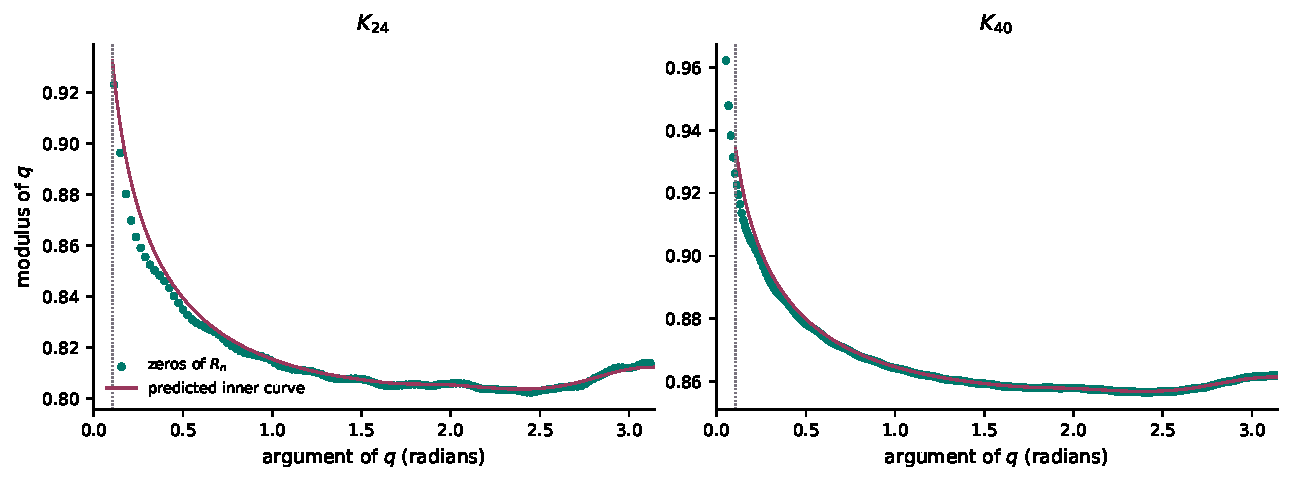
\includegraphics[width=0.97\textwidth]{figures/profile.pdf}
\caption{Zeros of $R_n$ in the upper half-plane for $n=24$ and $n=40$, plotted by argument and modulus, against the predicted inner curve $|q|=\exp(-b_n(\e^{\ii\theta}))$ of \eqref{bn}. The dotted line marks $\theta=\pi/30$, the end of the arc covered by Theorem~\ref{thm:bulk}. The minimum of the curve is near $\theta_*\approx2.39$. Zeros were computed with certified root isolation; the curve is a floating-point evaluation.}\label{fig:profile}
\end{figure}

\section{Notation and basic identities}\label{sec:notation}
This section defines the objects used throughout and records the identities on which the proofs rest.

\paragraph{Graphs and matroids.} For a connected loopless multigraph with $v\ge2$ vertices and $m$ edges put $r=v-1$ and $d=m-r$. For $K_n$ we write
\[
R_n=R_{K_n},\qquad N=\binom n2,\qquad d_n=N-n+1,\qquad N_k=\binom k2 .
\]
Thus $N$ is the degree of $R_n$ and $d_n$ is the number of its zeros other than the zero of order $n-1$ at $q=1$ (the \emph{nontrivial} zeros). We write $\T=\{|z|=1\}$, $\sigma$ for the uniform probability measure on $\T$, and $\mu_P=(\deg P)^{-1}\sum_{P(\zeta)=0}\delta_\zeta$ for the zero-counting measure of a polynomial $P$, with multiplicity.

\paragraph{The deformed exponential.} For $w\in\T$ let
\[
F_w(z)=\sum_{k\ge0}w^{-N_k}\frac{z^k}{k!}.
\]
This entire function is Macintyre's function $\mu_c(z)=\sum_kc^{N_k}z^k/k!$ with $c=\bar w$, in Waldvogel's notation \cite{Wald}. At $w=-1$ the signs of the coefficients have period four and $F_{-1}(z)=\cos z+\sin z$, whose zero of least modulus is $-\pi/4$; we write $a=\pi/4$. At $w=1$, $F_1=\exp$ has no zeros. Waldvogel's constant is
\begin{equation}\label{variational}
W_0=\min\{|z|:\ F_w(z)=0,\ w\in\T\}.
\end{equation}
The minimum exists by continuity and compactness, and $W_0\le a$. From now on we write $A=W_0$. When $F_w$ has a unique zero of least modulus and it is simple, we call it $\rho=\rho(w)$ and put
\begin{equation}\label{lambda}
\lambda(w)=-\frac{\rho F_w''(\rho)}{2F_w'(\rho)},\qquad \ell(w)=\Rea\lambda(w).
\end{equation}
At $w=-1$, $F''=-F$ gives $\lambda=0$. For $q=w\e^{-s}$ with $w\in\T$ and $\Rea s\ge0$ we use the centring
\begin{equation}\label{bn}
b_n(w)=\frac{\log((n-1)!)-n\log|\rho(w)|}{N+n\ell(w)},\qquad b_n=b_n(-1)=\frac{\log((n-1)!)-n\log a}{N}.
\end{equation}
Stirling's formula gives $nb_n(w)=2\log n-2(1+\log|\rho(w)|)+o(1)$, uniformly on compact sets of phases where $\rho$ is defined and continuous.

\paragraph{The exponential identity.} For fixed $q\ne0$ and $K\ge0$ let
\[
P_K(z;q)=\sum_{k=0}^{K}q^{-N_k}\frac{z^k}{k!}.
\]
Weight each edge present in a graph on $k$ labelled vertices by $(1-q)/q$; the total weight of all such graphs is $q^{-N_k}$, and taking the logarithm selects the connected ones. This gives the polynomial identity
\begin{equation}\label{egf}
R_n(q)=q^{N}\,n!\,\coef n\log P_n(z;q),
\end{equation}
which is Gilbert's formula \cite[eq.~(3)]{Gilbert} (see also \cite[eq.~(3.9)]{SS}). Expanding the logarithm over set partitions $\pi$ of the vertex set gives the partition formula \cite[\S2]{Gilbert}, \cite[eqs.~(3.48), (3.50)]{SS}
\begin{equation}\label{partition}
R_n(q)=\sum_{\pi}(-1)^{|\pi|-1}(|\pi|-1)!\,q^{e(\pi)},\qquad e(\pi)=\tfrac12\Bigl(n^2-\sum_{B\in\pi}|B|^2\Bigr),
\end{equation}
where $e(\pi)$ is the number of edges joining different blocks. Conditioning on the component of one vertex gives Gilbert's recurrence $R_n=1-\sum_{k=1}^{n-1}\binom{n-1}{k-1}q^{k(n-k)}R_k$, which the programs use.

\paragraph{Mallows--Riordan form.} Alsmeyer, Bostan, Raschel and Simon \cite[eq.~(2)]{ABRS} write
\[\log\sum_{k\ge0}\theta^{N_k}\frac{z^k}{k!}=\sum_{n\ge1}(\theta-1)^{n-1}J_n(\theta)\frac{z^n}{n!},\]
where the Mallows--Riordan polynomial $J_n$ has degree $d_n$ and positive coefficients. Putting $\theta=1/q$ in \eqref{egf} gives
\begin{equation}\label{MR}
R_n(q)=(1-q)^{n-1}q^{d_n}J_n(1/q).
\end{equation}
By \cite[Remark~2.2]{ABRS}, $J_n$ is positive on $[-1,\infty)$. Hence $R_n$ has no zero in $(-\infty,-1]$, and $R_n(-1)$ has the sign $(-1)^{d_n}$.

\section{Equidistribution on the unit circle}\label{sec:global}
This section proves the macroscopic statement: when the zeros, counted with multiplicity, become uniformly spread over the unit circle. Let $M$ be a loopless matroid of rank $r$ on $m\ge1$ elements, and let $R_M(q)$ be the probability that the surviving elements span $M$ when each element fails independently with probability $q$. For the cycle matroid of a connected graph this is $R_G$.

\begin{proposition}\label{prop:global}
Let $M_j$ be loopless matroids of positive rank $r_j$ on $m_j$ elements. The zero-counting measures of $R_{M_j}$ converge weakly to $\sigma$ if and only if $r_j/m_j\to0$. In particular, for connected loopless multigraphs with $v_j\ge2$ vertices and $m_j$ edges this happens exactly when $(v_j-1)/m_j\to0$, and it happens for $K_n$.
\end{proposition}

\begin{proof}
Let $T_M$ be the Tutte polynomial and $d=m-r$. Since $T_M(1,y)=\sum_{A\ \text{spanning}}(y-1)^{|A|-r}$, summing the probabilities of spanning surviving sets gives
\[
R_M(q)=(1-q)^rH(q),\qquad H(q)=q^{d}\,T_M(1,1/q).
\]
For graphs this is the identity in \cite[\S4.7]{BH}. The deletion--contraction recurrence shows by induction that $T_M$ has nonnegative integer coefficients. It also shows $T_M(1,0)\ge1$ for loopless $M$: if every element is a coloop then $T_M=x^m$; otherwise pick $e$ that is neither a loop nor a coloop, and $T_M(1,0)=T_{M\setminus e}(1,0)+T_{M/e}(1,0)\ge T_{M\setminus e}(1,0)$ with $M\setminus e$ loopless. In the spanning-set expansion only $A=E$ contributes to $y^d$, so $T_M(1,y)$ has degree $d$ with leading coefficient $1$. Hence $H$ has nonnegative integer coefficients, $H(0)=1$, leading coefficient $T_M(1,0)\ge1$, and $H(1)=T_M(1,1)=\tau(M)$, the number of bases. So $R_M$ has degree $m$, constant term $1$, leading coefficient of modulus at least $1$, and a zero of exact order $r$ at $q=1$.

For $P(z)=\sum_{k=0}^mc_kz^k$ with $c_0c_m\ne0$ put $L(P)=\log\bigl(\sum_k|c_k|/\sqrt{|c_0c_m|}\bigr)$. Hughes and Nikeghbali \cite[Theorems~1--3]{HN} prove, for deterministic polynomials, that the angular discrepancy of $\mu_P$ on any arc is $O(\sqrt{L(P)/m})$ (their Theorem~2, the Erd\H os--Tur\'an inequality) and that the proportion of zeros outside $\{1-\delta\le|z|\le(1-\delta)^{-1}\}$ is at most $2L(P)/(m\delta)$; in particular $\mu_{P_j}\to\sigma$ whenever $m_j\to\infty$ and $L(P_j)=o(m_j)$. Here
\[
L(R_M)\le r\log2+\log\tau(M)\le r\log2+\log\binom mr\le r\log\frac{2\e m}{r},
\]
which is $o(m)$ when $r/m\to0$ (and then $m\to\infty$). This proves sufficiency. Conversely, $\mu_{R_M}$ has an atom of mass exactly $r/m$ at $q=1$. If $\mu_{R_{M_j}}\to\sigma$, the portmanteau theorem applied to the closed set $\{1\}$ gives $\limsup r_j/m_j\le\sigma(\{1\})=0$.
\end{proof}

For $K_n$ the bound gives angular discrepancy $O(\sqrt{\log n/n})$ and mass $O(\log n/n)$ outside any fixed annulus about $\T$. These scales are far coarser than the individual-zero estimates below. The two extremes are realised by trees ($R=(1-q)^{n-1}$, all mass at $1$) and by two vertices joined by $m$ parallel edges ($R=1-q^m$, the $m$th roots of unity).

\section{Analytic tools}\label{sec:tools}
This section proves four lemmas used in all later sections: a zero-free disk, the exact half-degree split, a phase-uniform approximation by the deformed exponential, and the local model near an isolated smallest zero. Throughout, $K=\lfloor n/2\rfloor$, $q=w\e^{-s}$ with $w\in\T$, and $C,C',\ldots$ denote constants independent of $n$, $w$ and $s$.

\begin{lemma}[A zero-free disk]\label{lem:disk}
For every fixed $C>2\log2$,
\[
\sup_{|q|\le\exp(-(2\log n+C)/n)}|R_n(q)-1|\longrightarrow0 .
\]
\end{lemma}
\begin{proof}
In \eqref{partition} the one-block term is $1$. Mark a largest block and let $n-j$ be its size, $1\le j<n$. The number of ways to choose the marked block and an ordered set partition of the other $j$ vertices is at most $\binom nj j!\,2^{j-1}\le(2n)^j$ (list the $j$ vertices in some order and insert cuts), and this bounds the total weight $(|\pi|-1)!$ at this $j$. The crossing edges of the largest block give $e(\pi)\ge j(n-j)$, and $\sum|B|^2\le(n-j)n$ gives $e(\pi)\ge nj/2$. Put $\tau_n=(2\log n+C)/n$. For $j\le n/4$ use $e(\pi)\ge j(n-j)\ge3nj/4$: these terms sum to at most $\sum_{j\ge1}(2n\e^{-3n\tau_n/4})^j=O(n^{-1/2})$. For $j>n/4$ use $e(\pi)\ge nj/2$: these terms sum to at most $\sum_{j>n/4}(2\e^{-C/2})^j$, which tends to $0$ because $2\e^{-C/2}<1$.
\end{proof}

\begin{lemma}[The half-degree split]\label{lem:split}
For $q\ne0$,
\begin{align}
R_n(q)&=S_n(q)+B_n(q),\label{split}\\
S_n(q)&=q^{N}n!\,\coef n\log P_K(z;q),\qquad
B_n(q)=\sum_{j=0}^{n-K-1}(n)_j\,q^{j(2n-j-1)/2}\,\coef j P_K(z;q)^{-1},\nonumber
\end{align}
where $(n)_j=n!/(n-j)!$.
\end{lemma}
\begin{proof}
Write $P_n=P_K+V$, where $V$ contains only powers $z^k$ with $k\ge K+1$. Since $2(K+1)>n$, in $\log(P_K+V)=\log P_K+V/P_K-V^2/(2P_K^2)+\cdots$ every term with $V^2$ or higher has no $z^n$ coefficient. Hence $\coef n\log P_n=\coef n\log P_K+\coef n V/P_K$. Expanding $\coef n V/P_K=\sum_j\coef{n-j}V\cdot\coef jP_K^{-1}$ with $n-j\ge K+1$ and using $N-N_{n-j}=j(2n-j-1)/2$ gives $B_n$.
\end{proof}
The term with $j=0$ in $B_n$ is $1$, the term with $j=1$ is $-nq^{n-1}$ because $\coef1P_K^{-1}=-1$; so $B_n=1-nq^{n-1}+\cdots$ reproduces Gilbert's approximation \cite{Gilbert}. In words, $B_n$ collects configurations with one block of size larger than $n/2$, and $S_n$ those whose blocks all have size at most $n/2$.

\begin{lemma}[Phase-uniform approximation]\label{lem:uniform}
Fix $R'>0$, $C>0$ and an integer $p\ge0$. Uniformly for $w\in\T$, $|z|\le R'$ and complex $s$ with $0\le\Rea s\le(2\log n+C)/n$:
\begin{enumerate}
\item for every fixed $A_0>0$, the derivatives $\partial_s^jP_K(z;w\e^{-s})$, $j\le p$, are bounded, and
\[
P_K(z;w\e^{-s})=\sum_{j<p}\frac{s^j}{j!}\,D^jF_w(z)+O(|s|^{p}+n^{-A_0}),\qquad D=\tfrac{z^2}{2}\partial_z^2 ;
\]
\item if $0<r<\log2$ then $|\coef jP_K^{-1}|\le M_r\,r^{-j}$ for all $j$, with $M_r$ independent of $w$, $s$ and $n$;
\item if moreover $n\Rea s\ge(4/3+\varepsilon)\log n$ for a fixed $\varepsilon>0$, then $B_n(w\e^{-s})=1+o(1)$.
\end{enumerate}
\end{lemma}
\begin{proof}
(1) The $k$th summand of $P_K$ is $w^{-N_k}\e^{sN_k}z^k/k!$ and $\partial_s$ multiplies it by $N_k\le k^2$. Using $k!\ge(k/\e)^k$, after at most $p$ derivatives its modulus is at most $(1+k)^{2p}\bigl(\e R'\e^{k\Rea s/2}/k\bigr)^k$ for $k\ge1$. For $k\le n^{2/3}$ the factor $\e^{k\Rea s/2}$ is $1+o(1)$; for $n^{2/3}<k\le n/2$ the bracket is $O(n^{-1/6})$. So the derivatives are bounded uniformly. At $s=0$ the $j$th derivative is $D^j$ applied to the truncation of $F_w$, and the omitted tails are $O(n^{-A_0})$ for every $A_0$. Taylor's formula in $s$ with integral remainder gives the expansion. Only $\Rea s$ enters the bounds, so they hold for complex $s$ and all $w\in\T$.

(2) Since $P_K(z;q)$ depends on $(w,s)$ only through $q=w\e^{-s}$, we may replace $w$ by $w\e^{-\ii\Ima s}$ and assume that $s$ is real. For $|z|\le r<\log2$ one has $|F_w(z)-1|\le\e^{|z|}-1<1$ for every $w$, so by (1) with $p=1$ the function $P_K$ is bounded away from $0$ on $|z|\le r$ for large $n$, uniformly. Cauchy's estimate on $|z|=r$ gives the claim.

(3) In \eqref{split}, $n-(j+1)/2\ge3n/4-1$ for $j\le n-K-1$, so the terms with $j\ge1$ are bounded by $M_r\sum_{j\ge1}\bigl(nr^{-1}\e^{-(3n/4-1)\Rea s}\bigr)^j$, and the base is $O(n^{-\varepsilon'})$.
\end{proof}

\begin{lemma}[An isolated smallest zero]\label{lem:isolated}
Let $\Theta\subset\T$ be closed and $R>0$. Suppose that for every $w\in\Theta$, $F_w$ has no zero on $|z|=R$ and exactly one zero $\rho(w)$, counted with multiplicity, in $|z|<R$. Then $\rho$ is simple and continuous on $\Theta$, and the following hold uniformly for $w\in\Theta$ and for $s$ with $|\Ima s|=O(1/n)$ and $n\Rea s=2\log n+O(1)$.
\begin{enumerate}
\item $P_K(\cdot\,;w\e^{-s})$ has exactly one zero $\rho_n$ in $|z|<R$; it is simple and $\rho_n=\rho\,(1+\lambda s+O(|s|^2+n^{-3}))$.
\item $S_n(w\e^{-s})=-q^N(n-1)!\,\rho_n^{-n}\bigl(1+O(\kappa^n)\bigr)$ for some $\kappa<1$, with $q=w\e^{-s}$.
\item With $b_n(w)$ as in \eqref{bn} and $\eta_n(w)=-w^{N}(|\rho|/\rho)^n\exp[-\ii nb_n(w)\Ima\lambda]$, which has modulus one,
\begin{equation}\label{arc}
R_n\bigl(w\e^{-b_n(w)-t/N}\bigr)=1+\eta_n(w)\e^{-t}+o(1)
\end{equation}
uniformly for $w\in\Theta$ and $t$ in any bounded set of $\mathbb C$.
\end{enumerate}
\end{lemma}
\begin{proof}
Simplicity is the count, continuity follows from Rouch\'e's theorem, and compactness gives $\max_\Theta|\rho|<R$ and $\min_\Theta\min_{|z|=R}|F_w|>0$.

(1) By Lemma~\ref{lem:uniform}(1) with $p=2$, $P_K=F_w+s\,DF_w+O(|s|^2+n^{-3})$ on $|z|\le R+1$. Rouch\'e's theorem on $|z|=R$ gives exactly one zero $\rho_n$. Near $\rho$ one has $|F_w(z)|\ge c|z-\rho|$ uniformly, so $\rho_n-\rho=O(|s|+n^{-3})$; substituting into the expansion and using $DF_w(\rho)=\rho^2F_w''(\rho)/2$ gives the linear coefficient $-\rho F_w''(\rho)/(2F_w'(\rho))=\lambda$.

(2) The logarithmic derivative $P_K'/P_K$ has residue $1$ at $\rho_n$. Integrating $(P_K'/P_K)z^{-n}$ over $|z|=R$ and subtracting the residue gives $n\coef n\log P_K=-\rho_n^{-n}+O(R^{-n})$, since $P_K'/P_K$ is uniformly bounded on the contour. As $\max|\rho|<R$, the error is relatively $O(\kappa^n)$.

(3) Insert (1) into (2). Since $n|s|^2=O((\log n)^2/n)$,
$\rho_n^{-n}=\rho^{-n}\e^{-n\lambda s}(1+o(1))$, so $S_n=-w^{N}(n-1)!\,\rho^{-n}\e^{-(N+n\lambda)s}(1+o(1))$. Put $s=b_n(w)+t/N$. Then $n\lambda t/N=O(1/n)$ and $(N+n\lambda)b_n(w)=\log((n-1)!)-n\log|\rho|+\ii nb_n(w)\Ima\lambda$, which gives $S_n=\eta_n\e^{-t}(1+o(1))$. Stirling's formula shows that $nb_n(w)=2\log n+O(1)$, so Lemma~\ref{lem:uniform}(3) gives $B_n=1+o(1)$.
\end{proof}

\begin{lemma}[At most one zero in the disk of radius $\pi/4$]\label{lem:jensen}
For every $w\in\T$, $F_w$ has at most one zero, counted with multiplicity, in $|z|\le\pi/4$.
\end{lemma}
\begin{proof}
Suppose there were two. Jensen's formula at radius $2$, with $F_w(0)=1$, and the concavity of the logarithm give
\[
2\log\frac2a\le\frac1{2\pi}\int_0^{2\pi}\log|F_w(2\e^{\ii u})|\,du\le\frac12\log\frac1{2\pi}\int_0^{2\pi}|F_w(2\e^{\ii u})|^2du=\frac12\log\sum_{k\ge0}\frac{4^k}{(k!)^2}.
\]
The sum equals $11.30\ldots<12$ (the terms through $k=4$ give $11.22$ and the tail is below $0.1$), while $(2/a)^4=42.0\ldots>12$, a contradiction.
\end{proof}
Since $A\le a$, Lemma~\ref{lem:jensen} shows that at every phase $w$ attaining the minimum in \eqref{variational} the zero of least modulus is simple and unique, and that $\{w\}$ and $R=a$ satisfy the hypothesis of Lemma~\ref{lem:isolated} whenever $|\rho(w)|<a$.

\section{The negative real axis}\label{sec:negative}
This section counts and locates the negative real zeros. On the negative axis $w=-1$, $\rho=-a$, $\lambda=0$ and $b_n(-1)=b_n$.

\begin{theorem}\label{thm:negative}
As $n\to\infty$ the following hold.
\begin{enumerate}
\item Locally uniformly for $t\in\mathbb C$,
\[
R_n\bigl(-\exp(-b_n-t/N)\bigr)=1+(-1)^{d_n}\e^{-t}+o(1).
\]
Hence on every bounded region whose boundary avoids the zeros of the limit, the number of zeros in the $t$-coordinate eventually equals the number of zeros of $1+(-1)^{d_n}\e^{-t}$: the points $2\pi\ii k$ when $d_n$ is odd and $(2k+1)\pi\ii$ when $d_n$ is even.
\item For all sufficiently large $n$, $R_n$ has exactly one negative zero if $n\equiv0,3\pmod4$ and none otherwise. When it exists it is simple and equals $-\exp(-b_n-t_n/N)$ with $t_n=O((\log n)^2/n)$.
\item Let $t_0$ be a zero of the limit in (1) and $t_{n,0}$ the corresponding zero of $R_n$ in the $t$-coordinate. Then
\begin{equation}\label{correct}
t_{n,0}=t_0-\frac{a^2}{2}\,n\Bigl(b_n+\frac{t_0}{N}\Bigr)^2-\frac{2a^2}{3}\,nb_n^3+(-1)^{n-1}n\,\e^{-(n-1)b_n}+O(n^{-2}).
\end{equation}
\end{enumerate}
\end{theorem}
Note that $d_n$ is odd exactly when $n\equiv0,3\pmod 4$, and that $nb_n=2\log n-2(1+\log a)+o(1)$. So the real zero lies at distance $1+q_n\sim2\log n/n$ from $-1$, while consecutive complex zeros near the axis are $2\pi/N$ apart in angle. Exact integer computation confirms the count in part~(2) for every $2\le n\le24$ (Section~\ref{sec:certificates}); no explicit threshold is proved.

\begin{proof}
(1) Apply Lemma~\ref{lem:isolated} with $\Theta=\{-1\}$ and $R=1$: $\cos z+\sin z$ has the single zero $-a$ in $|z|<1$ (its other zeros have modulus at least $3a$). Here $\eta_n=-(-1)^N(-1)^n=(-1)^{d_n}$.

(2) By \eqref{MR} and the positivity of $J_n$ on $[-1,\infty)$, $R_n$ has no real zero in $(-\infty,-1]$, in $(0,1)$ or in $(1,\infty)$, and $R_n(0)=1$. So every real zero other than $q=1$ lies in $(-1,0)$. For $-1<q<0$ write $q=-\e^{-s}$ with $s>0$ and fix $C$ large. Lemma~\ref{lem:disk} excludes zeros with $ns\ge2\log n+C$. In the range $0<ns\le2\log n-C$ use the \emph{full} polynomial $P_n$ in \eqref{egf}. Fix $1<R'<3a$. The argument of Lemma~\ref{lem:uniform}(1) shows that $P_n(z;-\e^{-s})\to\cos z+\sin z$ uniformly on $|z|\le R'$ and on this range of $s$: for $k\le n/2$ as before, and for $n/2<k\le n$ the function $k\mapsto sk/2-\log k$ is convex, so $\e R'\e^{sk/2}/k$ is at most the larger of its endpoint values, which are $O(n^{-1/2})$ and $\e R'\e^{-C/2}$; choosing $C>2\log(2\e R')$ makes the omitted tail geometrically small. The residue argument of Lemma~\ref{lem:isolated}(2) on $|z|=1$ then shows that $n\coef n\log P_n$ equals $-\rho_n^{-n}+O(1)$, where $\rho_n$ is the unique zero in $|z|<1$, real by symmetry and tending to $-a$. Since $a<1$ this term dominates, and $R_n(-\e^{-s})$ has the constant sign $-(-1)^{N}(-1)^n=(-1)^{d_n}$ throughout the range. In the remaining strip $|ns-2\log n|\le C$, parts (1) and (2) of Lemma~\ref{lem:isolated} (with $\lambda=0$) give, uniformly for real $s$, $R_n(-\e^{-s})=1+o(1)+(-1)^{d_n}\e^{-N(s-b_n)}(1+o(1))$, with both error terms uniform separately. For even $d_n$ this is positive. For odd $d_n$ a zero needs $\e^{-N(s-b_n)}=1+o(1)$, that is $t=N(s-b_n)=o(1)$; Rouch\'e's theorem on a small circle in the $t$-plane gives exactly one zero counted with multiplicity, and complex conjugation makes it real.

(3) Lemma~\ref{lem:uniform}(1) with $p=4$ and the identity $\partial_s^jP_K|_{s=0}\to D^jF$ give the Taylor expansion of $\rho_n(s)$ at $w=-1$. Its coefficients are those of the zero of Macintyre's function $\mu_{-\e^{s}}$, whose expansion near $-\pi/4$ is Waldvogel's \cite[eq.~(3)]{Wald}: $z_0(-1-u)=\zeta+\zeta^3(u^2/2+u^3/6)+O(u^4)$ with $\zeta=-a$. With $u=\e^s-1$ this reads
\[
\frac{\rho_n(s)}{-a}=1+\frac{a^2}{2}s^2+\frac{2a^2}{3}s^3+O(|s|^4+n^{-3}).
\]
(The quadratic coefficient can also be checked directly: $D^2F=(z^4F''''+4z^3F'''+2z^2F'')/4$ equals $-z^3F'$ at $z=-a$.) In \eqref{split}, $\coef1P_K^{-1}=-1$, and the term with index $j$ is at most $M_r\bigl(r^{-1}n\,\e^{-(n-(j+1)/2)\Rea s}\bigr)^j$ by Lemma~\ref{lem:uniform}(2), for a fixed $r<\log2$. For $2\le j\le n/\log n$ the base is $r^{-1}n\e^{-n\Rea s}\e^{O(1)}=O(1/n)$, since $n\Rea s=2\log n+O(1)$; for larger $j$ the base is $O(n^{-1/2})$ as in Lemma~\ref{lem:uniform}(3). So the terms with $j\ge2$ sum to $O(n^{-2})$, and $B_n=1-nq^{n-1}+O(n^{-2})$. At a zero, $S_n=-B_n$. Taking logarithms on the branch near $t_0$ and using Lemma~\ref{lem:isolated}(2),
\[
t=t_0-n\log\frac{\rho_n(s)}{-a}-\log\bigl(1-nq^{n-1}\bigr)+O(n^{-2}),\qquad s=b_n+\frac tN .
\]
Here $q^{n-1}=(-1)^{n-1}\e^{-(n-1)s}$. Replacing $s$ by $b_n+t_0/N$ in the quadratic term and by $b_n$ elsewhere costs $O(n^{-2})$, because $t-t_0=O(\log^2 n/n)$, $N\asymp n^2$ and $n\e^{-(n-1)b_n}=O(1/n)$. This gives \eqref{correct}.
\end{proof}

Table~\ref{tab:finite} compares \eqref{correct} with zeros computed from the recurrence at 120 digits. Without the cubic term and the $t_0/N$ shift the error at $n=256$ is about $5\times10^{-3}$; with them it is between $40/n^2$ and $63/n^2$ for $63\le n\le256$, consistent with the $O(n^{-2})$ remainder. For $n\le32$ the omitted $O(n^{-2})$ terms are still comparable to the cubic term, and the refined formula is not yet more accurate than the first-order one.

\begin{table}[ht]
\centering\small
\begin{tabular}{rrrrrr}\toprule
$n$ & $n\bmod4$ & zero $t_{n,0}$ & first-order error & error of \eqref{correct} & $n^2\times$error\\\midrule
15 & 3 & $\phantom{-}0.0422350194$ & $0.0689$ & $0.196$ & 44.2\\
16 & 0 & $-0.5253031854$ & $0.122$ & $0.244$ & 62.5\\
31 & 3 & $-0.1585779198$ & $0.015$ & $0.0553$ & 53.2\\
32 & 0 & $-0.4581847228$ & $0.0129$ & $0.0553$ & 56.6\\
63 & 3 & $-0.1748111829$ & $0.0207$ & $0.0125$ & 49.5\\
64 & 0 & $-0.3222672082$ & $0.0208$ & $0.0117$ & 48.1\\
127 & 3 & $-0.1384017235$ & $0.0114$ & $0.00277$ & 44.6\\
128 & 0 & $-0.2109597112$ & $0.0114$ & $0.00260$ & 42.7\\
255 & 3 & $-0.0980080023$ & $0.00494$ & $0.000639$ & 41.6\\
256 & 0 & $-0.1339513463$ & $0.00494$ & $0.000610$ & 40.0\\
256 & 0 & $-0.1339294465+6.2827800361\,\ii$ & $0.00493$ & $0.000967$ & 63.4\\\bottomrule
\end{tabular}
\caption{The real zero ($t_0=0$) and, in the last row, the complex zero near $t_0=2\pi\ii$, in the coordinate $t=N(-\log(-q)-b_n)$, for orders with $d_n$ odd. ``First-order error'' is the error of \eqref{correct} without the cubic term and without the shift $t_0/N$. Floating computation at 120 digits; every computed root has recurrence residual below $10^{-60}$. The real zero is $q_n=-\exp(-b_n-t_{n,0}/N)$, for example $q_{256}=-0.96321157\ldots$.}\label{tab:finite}
\end{table}

\section{The inner radius}\label{sec:sharp}
This section proves the sharp asymptotic for the smallest modulus $h_n=\min\{|q|:R_n(q)=0\}$ and then, with the help of an interval certificate, identifies its directions.

\begin{theorem}\label{thm:sharp}
$-n\log h_n-2\log n\to-2(1+\log A)$, where $A=W_0$ is defined in \eqref{variational}.
\end{theorem}
Equivalently $h_n=1-\bigl(2\log n-2-2\log A+o(1)\bigr)/n$. With the enclosure of $A$ below, $-2(1+\log A)=-1.3917015\ldots$.

\begin{proof}
\emph{Lower bound for $-n\log h_n$.} Let $w_*$ attain the minimum in \eqref{variational}. By Lemma~\ref{lem:jensen} and $A\le a$, the zero $\rho(w_*)$ of modulus $A$ is simple and is the only zero of $F_{w_*}$ in $|z|\le a$. Choose $R$ with $A<R$ and $R$ smaller than the modulus of every other zero of $F_{w_*}$. Then Lemma~\ref{lem:isolated} applies with $\Theta=\{w_*\}$. The model $1+\eta_n\e^{-t}$ has a zero $t^{(n)}$ on the segment $\ii[-\pi,\pi]$, and on the circle $|t-t^{(n)}|=1/2$ its modulus has a positive lower bound independent of $n$. Rouch\'e's theorem therefore gives a zero of $R_n$ at $q=w_*\exp(-b_n(w_*)-t/N)$ with $|t-t^{(n)}|<1/2$. Its modulus is $\exp(-b_n(w_*)+O(1/N))$, so $-n\log h_n\ge nb_n(w_*)-o(1)=2\log n-2(1+\log A)+o(1)$.

\emph{Upper bound.} Fix $0<r<A$ and $\varepsilon>0$. By compactness $\min\{|F_w(z)|:w\in\T,|z|\le r\}>0$. Choose $C>|2(1+\log r)|+\varepsilon$, larger also than the constant of Lemma~\ref{lem:disk}. For real $s$ with $|ns-2\log n|\le C$, Lemma~\ref{lem:uniform}(1) gives $P_K\to F_w$ uniformly on $|z|\le r$ and in $w$, so $\log P_K$ is analytic and bounded on $|z|\le r$, and Cauchy's estimate gives
\[
|S_n(w\e^{-s})|\le C_r\,n!\,\e^{-Ns}r^{-n}.
\]
If in addition $ns\ge2\log n-2(1+\log r)+\varepsilon$, Stirling's formula shows that the logarithm of the right side is at most $-\varepsilon n/2+O(\log n)$. Together with $B_n=1+o(1)$ (Lemma~\ref{lem:uniform}(3)) this gives $R_n=1+o(1)$ there, uniformly in $w$. Beyond the strip Lemma~\ref{lem:disk} applies. Hence every zero satisfies $-n\log|q|<2\log n-2(1+\log r)+\varepsilon$ for large $n$. Letting $\varepsilon\downarrow0$ and $r\uparrow A$ proves the theorem.
\end{proof}

The proof uses only the definition \eqref{variational}. The finer statements below depend on a computer-assisted certificate, described in Section~\ref{sec:certificates}.

\begin{theorem}[computer-assisted]\label{thm:micro}
\begin{enumerate}
\item The constant satisfies \[0.73775075747822433247<A<0.73775075747822433248.\]
\item The minimum in \eqref{variational} is attained at exactly one conjugate pair of phases $w=\e^{\pm\ii\theta_*}$, with $2.39324227413489<\theta_*<2.39324227413490$ (about $137.12^\circ$). At these phases $\lambda$ is real and $\ell_*=\lambda(\e^{\ii\theta_*})$ satisfies $-0.2764138907713<\ell_*<-0.2764138907709$.
\item With $\ell_*$ as in (2),
\begin{equation}\label{micro}
h_n=\exp\!\left(-\frac{\log((n-1)!)-n\log A}{N+n\ell_*}\right)+o(n^{-2}).
\end{equation}
\item If $q_n$ is a zero of $R_n$ of modulus $h_n$, then every limit point of $\arg q_n$ is $\theta_*$ or $-\theta_*$. Since the zeros of $R_n$ are closed under conjugation, both values are attained.
\end{enumerate}
\end{theorem}
\begin{proof}
Parts (1) and (2), apart from the reality of $\lambda$, are the content of the certificate. Differentiating $F_w(\rho)=0$ in $\theta$ (with $w=\e^{\ii\theta}$), and using $\partial_\theta F_w=-\ii\,z^2F_w''/2$, gives $\rho'(\theta)/\rho=-\ii\lambda$. At a minimiser $\frac{d}{d\theta}\log|\rho|=\Rea(\rho'/\rho)=\Ima\lambda=0$, so $\lambda$ is real.

For (3) and (4), any closed set of phases avoiding $\pm\theta_*$ has, by compactness and (2), a zero-free disk for $F_w$ of radius $r>A$, uniformly on that set; the upper-bound argument of Theorem~\ref{thm:sharp} then excludes zeros of modulus $\le h_n$ in those directions for large $n$. Near $\theta_*$, Lemma~\ref{lem:isolated} applies on a closed neighbourhood $\Theta$ with $R=a$. For an innermost zero $q=w\e^{-s}$ with $w\in\Theta$ and real $s$, the split gives $|S_n|=|B_n|=1+o(1)$, hence
\[
(N+n\ell(\theta))s=\log((n-1)!)-n\log|\rho(\theta)|+o(1).
\]
The certificate gives $(|\rho|^2)''>0.31$ on an interval around $\theta_*$ containing every minimiser in $[0,\pi]$, so $\log|\rho(\theta)|-\log A\ge c\delta^2$ with $\delta=|\theta-\theta_*|$; the function $\ell$ is Lipschitz by the implicit function theorem. Writing $b_*$ for the exponent in \eqref{micro} and subtracting its defining equation,
\[
(N+n\ell(\theta))(s-b_*)\le-cn\delta^2+O(\delta\log n)+o(1)\le O\bigl((\log n)^2/n\bigr)+o(1)=o(1).
\]
So $-\log h_n\le b_*+o(n^{-2})$. Conversely \eqref{arc} at $\theta_*$ (where $\Ima\lambda=0$) places a zero at $s=b_*+t/N$ with $t$ within $o(1)$ of a purely imaginary model zero, by Rouch\'e on small circles, so $-\log h_n\ge b_*-o(n^{-2})$. Since $h_n$ is attained near $\pm\theta_*$ only, and zeros come in conjugate pairs, (4) follows.
\end{proof}

\begin{figure}[ht]
\centering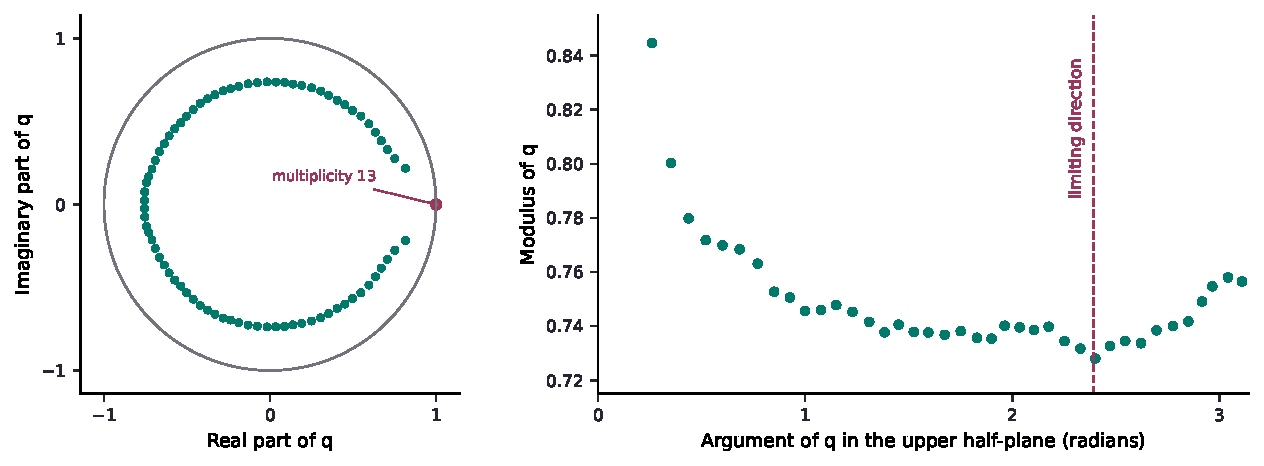
\includegraphics[width=0.94\textwidth]{figures/clique-roots.pdf}
\caption{The zeros of $R_{14}$. Left: the $78$ nontrivial zeros and the zero of order $13$ at $q=1$. Right: the zeros in the upper half-plane by argument and modulus; the dashed line is the limiting direction $\theta_*$ of the innermost zeros. Each nontrivial zero was isolated in its own disk of radius $10^{-22}$ (interval-certified).}\label{fig:k14}
\end{figure}

The negative axis is not extremal: there the constant is $-2(1+\log a)=-1.5168710\ldots<-1.3917015\ldots$, so the real zero is farther from the origin than the innermost complex zeros by about $0.125/n$ in modulus.

\section{The joint profile of angle and radius}\label{sec:bulk}
This section shows that, away from a small arc around $q=1$, the zeros sit on a single curve, one zero per angular gap of size $2\pi/N$. We record each zero $q_j$ ($j=1,\dots,N$, with multiplicity) by its argument $\arg q_j\in[0,2\pi)$ and its rescaled radial coordinate $H_n(q_j)=-n\log|q_j|-2\log n$.

\paragraph{The certified contours.} Let $J=\{\e^{\ii\theta}:\pi/30\le\theta\le59\pi/30\}$. The certificate of Section~\ref{sec:certificates} proves that the arc $[\pi/30,\pi]$ is a union of thirteen closed sub-arcs $\Theta_i$, with radii $R_i$, such that for every $w\in\Theta_i$ the function $F_w$ has no zero on $|z|=R_i$ and exactly one zero, counted with multiplicity, in $|z|<R_i$; the radii are $3/2$ on $[\pi/7,\pi]$ and between $1.85$ and $4.55$ on the twelve sub-arcs below $\pi/7$. By conjugation the same holds on $[\pi,59\pi/30]$. On overlaps the enclosed zeros coincide, so they define one continuous, simple zero $\rho(\theta)$ on $J$; it is the zero of least modulus of $F_{\e^{\ii\theta}}$. Put
\[
H(\theta)=-2\bigl(1+\log|\rho(\theta)|\bigr).
\]
At $\theta=\pi$, $H=-2(1+\log a)=-1.5169\ldots$; at $\theta_*$, $H=-2(1+\log A)=-1.3917\ldots$, its maximum; and $H$ decreases to about $-4.9$ at the ends of $J$, where $|\rho|\approx4.3$.

\begin{theorem}[computer-assisted]\label{thm:bulk}
On every closed interval $I\subset(\pi/30,59\pi/30)$ the finite measures
\[
\frac1N\sum_{\arg q_j\in I}\delta_{(\arg q_j,\,H_n(q_j))}\quad\text{converge weakly to}\quad\frac1{2\pi}\int_I\delta_{(\theta,H(\theta))}\,d\theta .
\]
The statement also holds for $I=[\pi/30,59\pi/30]$, where the limit has mass $29/30$.
\end{theorem}
The theorem gives the shape of the oval observed by Chang and Shrock \cite[\S6]{CS}: in the variable $q$, the zeros near direction $\theta$ lie at modulus $\exp(-b_n(\e^{\ii\theta})+o(n^{-2}))$. It says nothing about a vanishing proportion of zeros, which may lie anywhere, including outside the unit disk.

\begin{proof}
Lemma~\ref{lem:isolated} applies on each $\Theta_i$ with radius $R_i$, so \eqref{arc} holds uniformly for $w\in J$ and bounded $t$. Choose a continuous argument of $\rho(\theta)$ and lift the argument of $\eta_n$ to the real function
\[
\Psi_n(\theta)=\pi+N\theta-n\arg\rho(\theta)-nb_n(\e^{\ii\theta})\,\Ima\lambda(\theta).
\]
On $J$, $\rho$ is bounded away from $0$ and smooth with bounded derivatives, and differentiating \eqref{bn} gives $b_n=O(\log n/n)$ and $b_n'=O(1/n)$. Hence $\Psi_n'=N+O(n)>0$, and the points $\theta_j$ with $\Psi_n(\theta_j)\in\pi+2\pi\mathbb Z$ have consecutive gaps $(2\pi/N)(1+O(1/n))$.

At each $\theta_j$ the model in \eqref{arc} is $1-\e^{-t}$. On every circle $|t|=\varepsilon<1/2$ its modulus has a positive minimum independent of $j$, so the uniform version of Rouch\'e's theorem gives exactly one zero $q=\exp(\ii\theta_j-b_n(\e^{\ii\theta_j})-t_{n,j}/N)$ with $\max_j|t_{n,j}|\to0$. The angular extent of the image of $|t|\le1/2$ is $O(1/N)$ with constant below the gap, so these zeros are distinct for large $n$. By Stirling's formula, $nb_n(\e^{\ii\theta})-2\log n=H(\theta)+o(1)$ uniformly on $J$, so $H_n$ at these zeros equals $H(\theta_j)+o(1)$. The selected points with $\theta_j\in I$ therefore form Riemann sums for the limit measure; moving from centres $\theta_j\in I$ to zeros with argument in $I$ changes a bounded number of points.

Proposition~\ref{prop:global} gives total mass $|I|/(2\pi)+o(1)$ for all zeros with argument in $I$, because the end rays have limiting measure zero. The selected zeros already carry this mass, so the remaining zeros carry $o(1)$ against every bounded test function, whatever their radii. This proves the assertion for interior intervals, and exhausting $[\pi/30,59\pi/30]$ by interior intervals, with the same angular mass bound on the two small end intervals, gives the closed-arc statement.
\end{proof}

\section{The computer-assisted parts}\label{sec:certificates}
This section lists what is computed, by which method, and how to repeat it. Each statement is labelled as \emph{exact} (integer arithmetic), \emph{interval-certified} (outward-rounded interval or ball arithmetic) or \emph{floating} (high-precision illustration, not used in proofs).

\paragraph{Waldvogel's constant and the extremal phases (interval-certified).} Write $w=\e^{\ii\theta}$ and $z=r\e^{\ii\phi}$; conjugation reduces to $0\le\theta\le\pi$. The series $F_w$ is truncated at degree $25$; for $r\le1$ the tail is at most $2/26!$. On a box with half-widths $h$ in $\theta$ and $2h$ in $\phi$, the $k$th term changes phase by at most $(N_k+2k)h$, and its error after linearisation is at most $r^k(N_k+2k)^2h^2/(2\,k!)$. A box is discarded when the real or the imaginary part is separated from zero by the linear variation plus this remainder; near tangencies the test is applied to the determinant with the $\phi$-derivative, which removes the linear $\phi$ term. Failed boxes are split into four.
\begin{itemize}
\item At $r=0.73775075747822433247$ all phases are excluded (958 terminal boxes, depth at most 37). Since $F_1=\exp$ has no zeros and the zero count inside the circle is constant in $\theta$, no $F_w$ has a zero in this closed disk: this is the lower bound in Theorem~\ref{thm:micro}(1).
\item At one phase, a Rouch\'e disk of radius $10^{-23}$ about the point
\[z_0=-0.7330525232968298\ldots+0.0831274819048705\ldots\,\ii\]
contains a zero of modulus below $0.73775075747822433248$. This is the upper bound.
\item A cover of the radial band between the two bounds (355 boxes, depth at most 14) confines every minimiser with $0\le\theta\le\pi$ to $2.39224\le\theta\le2.39425$, $3.02767\le\phi\le3.02968$. On this patch a Rouch\'e disk of radius $0.002$ contains exactly one simple zero for every $\theta$ in the interval, implicit differentiation with tail bounds gives $(|\rho|^2)''>0.31$, and the signs of the derivative at $2.39324227413489$ and $2.39324227413490$ bracket the unique minimiser. The enclosure of $\ell_*$ is computed at the bracketed minimiser.
\end{itemize}
The same geometric tests were run with two arithmetic backends written independently: an integer interval arithmetic at $2^{-176}$ resolution and a second integer arithmetic with a rational Machin bound for $\pi$ (the curvature lower bounds obtained are $0.312$ and $0.320$); both reproduce every line, and a third run uses \texttt{mpmath.iv}. The backends share the subdivision scheme, so they check the arithmetic, not the geometry.

\paragraph{The contours for Theorem~\ref{thm:bulk} (interval-certified).} On $[\pi/7,\pi]$ the same box test at radius $3/2$ (tail $2(3/2)^{26}/26!$) excludes zeros on $|z|=3/2$ (365 boxes, depth at most 6); at $\theta=\pi$ the disk contains exactly one zero of $\cos z+\sin z$. Below $\pi/7$ a separate program in Arb ball arithmetic \cite{Arb} uses the truncation at degree $60$ with tail $2R^{61}/61!$, the same first-order box test with its second-order remainder (on the circle), a first-order test in the variable $\log z$ with remainder $|x|^2\e^{|x|}/2$ (on annuli), and twelve sub-arcs whose endpoints are $\theta=\pi/7,\pi/9,\pi/11,\ldots,\pi/19,\pi/20,\pi/22,\ldots,\pi/30$, with radii increasing from $37/20$ to $91/20$. On each sub-arc it excludes zeros on the circle $|z|=R_i$ for every phase, and at each junction phase it excludes zeros from the closed annulus between the two neighbouring radii, so that the count of enclosed zeros, which is constant along each sub-arc, is passed from one sub-arc to the next. The exact sub-arcs, radii and box counts (between $58$ and $4176$ boxes per sub-arc) are recorded in the output file. As negative controls, the same program fails, as it should, on the circle $|z|=8/5$ over $[\pi/9,\pi/7]$, which a zero crosses, and on the annulus $13/10\le|z|\le3/2$ at $\theta=\pi/7$, which contains a zero.

\paragraph{Exact and floating checks.} The recurrence and direct enumeration of all labelled spanning subgraphs agree through $K_6$ (26{,}704 connected spanning subgraphs of $K_6$). Integer Descartes-rule subdivisions, with a Sturm fallback, count the real zeros of $R_n$ for $2\le n\le24$ (exact): none in $(-\infty,-1]$, and one in $(-1,0)$ exactly when $n\equiv0,3\pmod4$. Table~\ref{tab:finite} and the transition-window checks are floating, at 80--150 digits with cross-precision comparison. The zeros in Figure~\ref{fig:profile} are isolated by Arb; each zero of $K_{14}$ in the program \texttt{plot\_roots.py} is isolated in its own disk of radius $10^{-22}$.

\paragraph{Reproduction.} All programs are in the accompanying repository and run in minutes with Python 3.12, \texttt{mpmath} 1.3.0, \texttt{sympy} 1.14.0 and \texttt{python-flint} 0.7.1. The certificate programs stop with an error, and print no success line, if any inequality fails; they do not rely on \texttt{assert} statements.

\section{Scope and open problems}\label{sec:scope}
This section states what the results do not cover.
\begin{itemize}
\item \emph{Every order.} The negative-axis count is proved for all sufficiently large $n$ and checked exactly for $n\le24$. All estimates are explicit in principle, so an effective threshold combined with a finite computation would give the count for every $n$; we have not carried this out.
\item \emph{Zeros outside the disk.} Theorems~\ref{thm:sharp}--\ref{thm:bulk} control the inner edge and $29/30$ of the zeros; they allow $o(N)$ exceptional zeros anywhere. Buys's Question~4.1, whether every nontrivial zero of $R_n$ lies in the open unit disk, remains open; after the substitution $y=1/q$ it is Sokal's conjecture that the generating polynomials of connected graphs have no zeros with $|y|<1$, together with his suspicion that $y=1$ is the only zero on $|y|=1$ \cite[slide~8, Big Conjecture~\#3]{Sokal}. For general graphs, Bencs, Piombi and Regts \cite{BPR} show that reliability zeros of modulus larger than $1$ occur in essentially every direction.
\item \emph{The arc near $q=1$.} Numerically the smallest zero of $F_w$ stays simple and separated as $\theta\to0$, with $|\rho(\theta)|$ growing roughly like $0.45/\theta$, so Theorem~\ref{thm:bulk} should hold on every closed arc avoiding $q=1$; each fixed arc is a finite certificate of the kind described above, but the full statement needs an analytic argument as $\theta\to0$, where the problem passes into the connectivity window of the real random graph.
\item \emph{The inner radius over all graphs.} Brown and DeGagn\'e \cite{BD19b} showed that among all graphs on $n\ge3$ vertices the reliability zero of smallest modulus belongs to the cycle $C_n$. Theorem~\ref{thm:sharp} concerns the dense family $K_n$ instead.
\item \emph{Related announced work.} Scott and Sokal \cite[\S3.4.1 and ref.~55]{SS} announced a study of the asymptotic behaviour at complex parameters of the Tutte polynomials of the complete graphs, based on the partition formulae used in Lemma~\ref{lem:disk}.
\end{itemize}

\section*{AI-use statement}
This paper was prepared with substantial assistance from AI systems, which drafted the text and the programs and checked the proofs. The mathematical statements are supported by the proofs given here and by the computations described in Section~\ref{sec:certificates}. The paper has not been refereed.

\begin{thebibliography}{99}\small
\bibitem{ABRS} G. Alsmeyer, A. Bostan, K. Raschel and T. Simon, Persistence for a class of order-one autoregressive processes and Mallows--Riordan polynomials, \emph{Advances in Applied Mathematics} 150 (2023), 102555. \url{https://doi.org/10.1016/j.aam.2023.102555}
\bibitem{Arb} F. Johansson, Arb: efficient arbitrary-precision midpoint-radius interval arithmetic, \emph{IEEE Transactions on Computers} 66 (2017), 1281--1292. \url{https://doi.org/10.1109/TC.2017.2690633}
\bibitem{BH} S. Backman and S. Hopkins, Fourientations and the Tutte polynomial, \emph{Research in the Mathematical Sciences} 4 (2017), 18. \url{https://doi.org/10.1186/s40687-017-0107-z}
\bibitem{BPR} F. Bencs, C. Piombi and G. Regts, On the complex zeros and the computational complexity of approximating the reliability polynomial, arXiv:2512.11504 (2025). \url{https://arxiv.org/abs/2512.11504}
\bibitem{BD19b} J. I. Brown and C. D. C. DeGagn\'e, All terminal reliability roots of smallest modulus, arXiv:1906.02359 (2019). \url{https://arxiv.org/abs/1906.02359}
\bibitem{BM} J. I. Brown and I. McMullin, On the real reliability roots of graphs, \emph{Discrete Applied Mathematics} 388 (2026), 174--180. \url{https://doi.org/10.1016/j.dam.2026.03.037}
\bibitem{Buys} P. Buys, Density of reliability roots of simple graphs in the unit disk, arXiv:2604.07541 (2026). \url{https://arxiv.org/abs/2604.07541}
\bibitem{CS} S.-C. Chang and R. Shrock, Reliability polynomials and their asymptotic limits for families of graphs, \emph{Journal of Statistical Physics} 112 (2003), 1019--1077. \url{https://doi.org/10.1023/A:1024663508526}
\bibitem{Gilbert} E. N. Gilbert, Random graphs, \emph{The Annals of Mathematical Statistics} 30 (1959), 1141--1144. \url{https://doi.org/10.1214/aoms/1177706098}
\bibitem{HN} C. P. Hughes and A. Nikeghbali, The zeros of random polynomials cluster uniformly near the unit circle, \emph{Compositio Mathematica} 144 (2008), 734--746. \url{https://doi.org/10.1112/S0010437X07003302}
\bibitem{Omar} M. Omar, Real reliability roots of simple graphs are dense, arXiv:2604.03530 (2026). \url{https://arxiv.org/abs/2604.03530}
\bibitem{RS} G. Royle and A. D. Sokal, The Brown--Colbourn conjecture on zeros of reliability polynomials is false, \emph{Journal of Combinatorial Theory, Series B} 91 (2004), 345--360. \url{https://doi.org/10.1016/j.jctb.2004.03.008}
\bibitem{SS} A. D. Scott and A. D. Sokal, Some variants of the exponential formula, with application to the multivariate Tutte polynomial (alias Potts model), \emph{S\'eminaire Lotharingien de Combinatoire} 61A (2009), B61Ae; arXiv:0803.1477. \url{https://arxiv.org/abs/0803.1477}
\bibitem{Sokal} A. D. Sokal, The deformed exponential function and a plethora of related things, seminar slides, Mark Kac Seminar, Utrecht, 10 June 2011. \url{https://www.mark-kac-seminar.nl/2010-2011/2011-June-Sokal.pdf}
\bibitem{Wald} J. Waldvogel, The Whittaker constant, in \emph{Konstruktive Verfahren der komplexen Analysis}, Tagungsbericht 35/1983, Mathematisches Forschungsinstitut Oberwolfach (1983), 4--5. \url{https://oda.mfo.de/handle/mfo/1017}
\end{thebibliography}
\end{document}
